%===============================================================================
% LaTeX sjabloon voor de bachelorproef toegepaste informatica aan HOGENT
% Meer info op https://github.com/HoGentTIN/latex-hogent-report
%===============================================================================

\documentclass[dutch,dit,thesis]{hogentreport}

% - If necessary, replace the option `dit`' with your own department!
%   Valid entries are dbo, dbt, dgz, dit, dlo, dog, dsa, soa
% - If you write your thesis in English (remark: only possible after getting
%   explicit approval!), remove the option "dutch," or replace with "english".

\usepackage{lipsum} % For blind text, can be removed after adding actual content

%% Pictures to include in the text can be put in the graphics/ folder
\graphicspath{{graphics/}}

%% For source code highlighting, requires pygments to be installed
%% Compile with the -shell-escape flag!
%% \usepackage[section]{minted}
%% If you compile with the make_thesis.{bat,sh} script, use the following
%% import instead:
\usepackage[section,outputdir=../output]{minted}
\usemintedstyle{solarized-light}
\definecolor{bg}{RGB}{253,246,227} %% Set the background color of the codeframe

%% Change this line to edit the line numbering style:
\renewcommand{\theFancyVerbLine}{\ttfamily\scriptsize\arabic{FancyVerbLine}}

%% Macro definition to load external java source files with \javacode{filename}:
\newmintedfile[javacode]{java}{
    bgcolor=bg,
    fontfamily=tt,
    linenos=true,
    numberblanklines=true,
    numbersep=5pt,
    gobble=0,
    framesep=2mm,
    funcnamehighlighting=true,
    tabsize=4,
    obeytabs=false,
    breaklines=true,
    mathescape=false
    samepage=false,
    showspaces=false,
    showtabs =false,
    texcl=false,
}

% Other packages not already included can be imported here

%%---------- Document metadata -------------------------------------------------
\author{Warre Vandenhoucke}
\supervisor{Dhr. L. Smits}
\cosupervisor{Dhr. J. Decubber}
\title
    {Efficiënte integratie van kalender-API's in software: Een gebruikersgerichte benadering}
\academicyear{\advance\year by -1 \the\year--\advance\year by 1 \the\year}
\examperiod{2}
\degreesought{\IfLanguageName{dutch}{Professionele bachelor in de toegepaste informatica}{Bachelor of applied computer science}}
\partialthesis{false} %% To display 'in partial fulfilment'
%\institution{Internshipcompany BVBA.}

%% Add global exceptions to the hyphenation here
\hyphenation{back-slash}

%% The bibliography (style and settings are  found in hogentthesis.cls)
\addbibresource{bachproef.bib}            %% Bibliography file
\addbibresource{../voorstel/voorstel.bib} %% Bibliography research proposal
\defbibheading{bibempty}{}

%% Prevent empty pages for right-handed chapter starts in twoside mode
\renewcommand{\cleardoublepage}{\clearpage}

\renewcommand{\arraystretch}{1.2}

%% Content starts here.
\begin{document}

%---------- Front matter -------------------------------------------------------

\frontmatter

\hypersetup{pageanchor=false} %% Disable page numbering references
%% Render a Dutch outer title page if the main language is English
\IfLanguageName{english}{%
    %% If necessary, information can be changed here
    \degreesought{Professionele Bachelor toegepaste informatica}%
    \begin{otherlanguage}{dutch}%
       \maketitle%
    \end{otherlanguage}%
}{}

%% Generates title page content
\maketitle
\hypersetup{pageanchor=true}

%%=============================================================================
%% Voorwoord
%%=============================================================================

\chapter*{\IfLanguageName{dutch}{Woord vooraf}{Preface}}%
\label{ch:voorwoord}

Kalendersoftware is al lang belangrijk voor zowel persoonlijk gebruik als voor bedrijven. Met de groei van digitale tools om ons leven en werk te organiseren, is goede kalendersoftware nog belangrijker geworden. Maar met zoveel verschillende bedrijven die kalendersoftware maken, is het soms lastig om de beste te kiezen. In mijn bachelorproef, getiteld "Efficiënte Integratie van Kalender-API's in Software: Een Gebruikersgerichte Benadering", onderzoek ik hoe je verschillende soorten kalendersoftware goed samen kunt laten werken in een applicatie.

Ik heb dit onderwerp gekozen omdat het bedrijf TurnUp en ik geïnteresseerd zijn in het makkelijker maken van kalendersoftware in een nieuwe app die ze ontwerpen. Dit onderzoek probeert uit te vinden hoe ze verschillende kalenderprogramma's het beste kunnen combineren om alles makkelijker en beter te maken voor de gebruiker. Dit is vooral belangrijk nu er steeds meer verschillende kalendertools zijn en er meer vraag is naar oplossingen die beter samenwerken.

Ik wil mijn copromotor, Jona Decubber, hartelijk bedanken voor zijn deskundige begeleiding en inzichten die van groot belang waren voor mijn onderzoek. Zijn hulp was cruciaal om door de complexe onderwerpen heen te werken.

Ook wil ik mijn familie heel erg bedanken voor hun constante steun en de nuttige feedback die ze mij gegeven hebben tijdens dit proces. Hun aanmoediging hielp mij door moeilijke tijden heen.

Dit onderzoek kijkt naar verschillende aspecten van het ontwikkelen en integreren van software, en ik hoop dat de resultaten nuttig zullen zijn voor professionals en anderen die geïnteresseerd zijn in het verbeteren van kalendersystemen. De bevindingen in deze scriptie kunnen hopelijk helpen om beter te begrijpen hoe we kalendersoftware kunnen verbeteren voor gebruikers in allerlei verschillende situaties.


%%=============================================================================
%% Samenvatting
%%=============================================================================

% thesis) synthese van het document.
%
% Een goede abstract biedt een kernachtig antwoord op volgende vragen:
%
% 1. Waarover gaat de bachelorproef?
% 2. Waarom heb je er over geschreven?
% 3. Hoe heb je het onderzoek uitgevoerd?
% 4. Wat waren de resultaten? Wat blijkt uit je onderzoek?
% 5. Wat betekenen je resultaten? Wat is de relevantie voor het werkveld?
%
% Daarom bestaat een abstract uit volgende componenten:
%
% - inleiding + kaderen thema
% - probleemstelling
% - (centrale) onderzoeksvraag
% - onderzoeksdoelstelling
% - methodologie
% - resultaten (beperk tot de belangrijkste, relevant voor de onderzoeksvraag)
% - conclusies, aanbevelingen, beperkingen
%
% LET OP! Een samenvatting is GEEN voorwoord!

%%---------- Nederlandse samenvatting -----------------------------------------
%
% Nederlandse samenvatting invoegen. Haal daarvoor onderstaande code uit
% commentaar.
% Wie zijn bachelorproef in het Nederlands schrijft, kan dit negeren, de inhoud
% wordt niet in het document ingevoegd.

% \IfLanguageName{english}{%
% \selectlanguage{dutch}
% \chapter*{Samenvatting}
% \lipsum[1-4]
% \selectlanguage{english}
% }{}

%%---------- Samenvatting -----------------------------------------------------
% De samenvatting in de hoofdtaal van het document

\chapter*{\IfLanguageName{dutch}{Samenvatting}{Abstract}}

Deze bachelorproef richt zich op de integratie van diverse kalender-API's zoals Google Calendar, Calendly, en Microsoft Calendar in één uniforme applicatie en evalueert de impact daarvan op de gebruikerservaring. Het onderzoek stelt als doel om nieuwe methoden te ontwikkelen die zowel de efficiëntie als de gebruiksvriendelijkheid van deze integratie verbeteren, een uitdaging die steeds relevanter wordt naarmate meer organisaties streven naar een geïntegreerde digitale werkomgeving.

De methodologie van dit onderzoek omvat het ontwikkelen van een Proof of Concept (PoC), die gebruik maakt van moderne webtechnologieën zoals ReactJS, samen met backend-integraties via Node.js. De PoC implementeert functionele verbindingen met de genoemde kalenderdiensten, en biedt een real-time dashboard voor het beheren en synchroniseren van kalenderdata over deze verschillende platforms heen.

Uit de analyse van de gebruikerstesten en technische evaluaties blijkt dat de integratie van de kalender-API's significant bijdraagt aan een verbeterde gebruikerservaring door de interactie en dataconsistentie te vereenvoudigen. Echter, de studie identificeert ook uitdagingen zoals prestatiebeperkingen en complexiteit in data synchronisatie, die de algehele effectiviteit kunnen beïnvloeden.

De resultaten van dit onderzoek bieden waardevolle inzichten voor ontwikkelaars en organisaties zoals TurnUp, die streven naar efficiëntere en gebruikersvriendelijkere integratiesystemen. De studie benadrukt het belang van zorgvuldige planning en het testen van interface ontwerp om te zorgen voor een naadloze integratie-ervaring.

Toekomstig werk kan zich richten op het uitbreiden van de functionaliteit van de PoC, het verbeteren van de prestaties en het verder personaliseren van de gebruikersinterface. Ook kan verder onderzoek naar geavanceerde authenticatie- en beveiligingsprotocollen voor API-integraties nuttig zijn om de betrouwbaarheid en veiligheid van de geïntegreerde systemen te waarborgen.


%---------- Inhoud, lijst figuren, ... -----------------------------------------

\tableofcontents

% In a list of figures, the complete caption will be included. To prevent this,
% ALWAYS add a short description in the caption!
%
%  \caption[short description]{elaborate description}
%
% If you do, only the short description will be used in the list of figures

\listoffigures

% If you included tables and/or source code listings, uncomment the appropriate
% lines.
%\listoftables
%\listoflistings

% Als je een lijst van afkortingen of termen wil toevoegen, dan hoort die
% hier thuis. Gebruik bijvoorbeeld de ``glossaries'' package.
% https://www.overleaf.com/learn/latex/Glossaries

%---------- Kern ---------------------------------------------------------------

\mainmatter{}

% De eerste hoofdstukken van een bachelorproef zijn meestal een inleiding op
% het onderwerp, literatuurstudie en verantwoording methodologie.
% Aarzel niet om een meer beschrijvende titel aan deze hoofdstukken te geven of
% om bijvoorbeeld de inleiding en/of stand van zaken over meerdere hoofdstukken
% te verspreiden!

%%=============================================================================
%% Inleiding
%%=============================================================================

\chapter{\IfLanguageName{dutch}{Inleiding}{Introduction}}%
\label{ch:inleiding}

In een wereld waar afspraken een cruciale rol spelen in zowel het persoonlijke als zakelijke leven, is kalendersoftware onmisbaar geworden. Of het nu gaat om het plannen van vergaderingen, het bijhouden van deadlines of het beheren van persoonlijke verplichtingen, betrouwbare en efficiënte kalendersystemen zijn essentieel. Echter, door de verscheidenheid aan beschikbare kalendersoftware, elk met hun eigen unieke kenmerken en integratiemethoden, staan gebruikers en bedrijven voor de uitdaging om deze systemen op een naadloze manier te combineren en beheren.

In deze bachelorproef wordt de focus gelegd op de integratie van verschillende kalender-API's in softwareapplicaties. Het doel is om te onderzoeken hoe deze integraties de gebruikerservaring beïnvloeden en om innovatieve methoden te ontwikkelen die de efficiëntie en gebruiksvriendelijkheid verbeteren. Door de toenemende behoefte aan gecentraliseerde en efficiënte oplossingen voor kalenderbeheer, vormt dit onderzoek een belangrijke stap richting de optimalisatie van kalendersystemen in een breed scala aan toepassingen.

In samenwerking met TurnUp, een bedrijf dat zich inzet voor het oplossen van het wereldwijde probleem van no-shows en het bevorderen van een cultuur van punctualiteit en betrouwbaarheid, richt dit onderzoek zich op het ontwikkelen van een oplossing die niet alleen technische uitdagingen aanpakt, maar ook bijdraagt aan een verbeterde gebruikservaring.

\section{\IfLanguageName{dutch}{Probleemstelling}{Problem Statement}}%
\label{sec:probleemstelling}
\subsection{TurnUp}
TurnUp heeft als missie om de manier waarop de wereld omgaat met afspraken te revolutioneren door het wereldwijde probleem van no-shows aan te pakken \autocite{TurnUp2024}. Het bedrijf streeft ernaar om de uitdagingen en inefficiënties die gepaard gaan met gemiste afspraken te elimineren, en om zowel individuen als bedrijven te helpen het maximale uit geplande afspraken te halen.

Door middel van innovatieve oplossingen en geavanceerde technologie wil TurnUp een wereldwijde cultuur van betrouwbaarheid, punctualiteit en naadloze afsprakenervaringen creëren. Het bedrijf brengt een diverse gemeenschap van gebruikers, bedrijven en dienstverleners samen om een netwerk te vormen waarin afspraken niet slechts momenten zijn, maar kansen voor waardevolle verbindingen en samenwerkingen.

TurnUp ziet een toekomst voor zich waarin elke geplande interactie wordt gerespecteerd en gewaardeerd, en bijdraagt aan de groei en het succes van zowel individuen als organisaties. Door het probleem van no-shows op wereldwijde schaal aan te pakken, wil TurnUp een blijvende impact hebben op productiviteit, klanttevredenheid en algemeen welzijn.

\subsection{\IfLanguageName{dutch}{Probleem}{Problem}}
TurnUp zal om aan deze missie te werken, in de toekomst gebruik maken van diverse kalenderprogramma's die ze willen integreren in hun eigen kalendersoftware om alle data te centraliseren. Deze gecentraliseerde data zal gemakkelijker toegankelijk zijn voor toekomstig gebruik. Deze integratie kan echter niet zomaar gebeuren aangezien de verschillende softwarepakketten vaak andere manieren hebben van integreren. Dit onderzoek richt zich op het evalueren van de invloed van deze integratie op de gebruikerservaring en het identificeren van innovatieve benaderingen om deze integratie te optimaliseren.
Wanneer het onderzoek is afgewerkt kunnen zij verder aan de slag gaan met de integratie en implementatie van hun kalendersysteem.
Voor andere bedrijven die ook gebruik maken van een of meerdere kalenderapplicaties, kan dit onderzoek ook interessant zijn.

\section{\IfLanguageName{dutch}{Onderzoeksvraag}{Research question}}%
\label{sec:onderzoeksvraag}

Hoe beïnvloedt de integratie van verschillende kalender-API's de gebruikerservaring van ontwikkelaars in softwareapplicaties, en welke innovatieve benaderingen kunnen worden ontwikkeld om de efficiëntie en gebruiksvriendelijkheid van deze integratie te verbeteren?

\section{\IfLanguageName{dutch}{Onderzoeksdoelstelling}{Research objective}}%
\label{sec:onderzoeksdoelstelling}

Het doel van dit onderzoek is om de impact van de integratie van verschillende kalender-API's op de gebruikerservaring te evalueren en om nieuwe methoden te ontwikkelen die de efficiëntie en gebruiksvriendelijkheid van deze integratie verbeteren.

\section{\IfLanguageName{dutch}{Opzet van deze bachelorproef}{Structure of this bachelor thesis}}%
\label{sec:opzet-bachelorproef}

% Het is gebruikelijk aan het einde van de inleiding een overzicht te
% geven van de opbouw van de rest van de tekst. Deze sectie bevat al een aanzet
% die je kan aanvullen/aanpassen in functie van je eigen tekst.

De rest van deze bachelorproef is als volgt opgebouwd:

In Hoofdstuk~\ref{ch:stand-van-zaken} wordt een overzicht gegeven van de stand van zaken binnen het onderzoeksdomein, op basis van een literatuurstudie.

In Hoofdstuk~\ref{ch:methodologie} wordt de methodologie toegelicht en worden de gebruikte onderzoekstechnieken besproken om een antwoord te kunnen formuleren op de onderzoeksvragen.

In Hoofdstuk~\ref{ch:proof-of-concept} wordt de proof of concept besproken. Hoe de applicaties zijn opgebouwd en wat hiervoor werd gebruikt.

In Hoofdstuk~\ref{ch:analyse-testen} worden de resultaten van de proof of concept besproken.

In Hoofdstuk~\ref{ch:conclusie}, tenslotte, wordt de conclusie gegeven en een antwoord geformuleerd op de onderzoeksvraag. Daarbij wordt ook een aanzet gegeven voor toekomstig onderzoek binnen dit domein.
\chapter{\IfLanguageName{dutch}{Stand van zaken}{State of the art}}%
\label{ch:stand-van-zaken}

% Tip: Begin elk hoofdstuk met een paragraaf inleiding die beschrijft hoe
% dit hoofdstuk past binnen het geheel van de bachelorproef. Geef in het
% bijzonder aan wat de link is met het vorige en volgende hoofdstuk.

% Pas na deze inleidende paragraaf komt de eerste sectiehoofding.
\section{Inleiding}

De evolutie van kalendersoftware heeft een significante transformatie ondergaan sinds de dagen van fysieke kalenders. In het verleden was men beperkt tot handgeschreven notities en afspraken in papieren agenda's, wat vele beperkingen met zich meebracht, voornamelijk op het gebied van toegankelijkheid en flexibiliteit. Met de opkomst van digitale technologieën zijn deze traditionele methoden grotendeels vervangen door digitale kalenders, die een reeks voordelen bieden die verder gaan dan eenvoudig gemak.

\subsection{Voordelen van Digitale Kalenders}
Digitale kalenders bieden ongeëvenaarde voordelen die hun wijdverbreide adoptie hebben aangedreven:
\begin{itemize}
    \item \textbf{Toegankelijkheid:} Digitale kalenders kunnen overal en altijd worden geraadpleegd, mits er internetverbinding is, waardoor gebruikers hun schema's gemakkelijker kunnen beheren en aanpassen.
    \item \textbf{Synchronisatie:} Gebruikers kunnen afspraken en evenementen synchroniseren over meerdere apparaten en platforms heen, wat zorgt voor consistentie en helpt bij het voorkomen van planningsconflicten.
    \item \textbf{Integratie:} Integratie met andere digitale tools en applicaties verhoogt de functionaliteit, zoals het automatisch instellen van herinneringen en het delen van afspraken met anderen.
\end{itemize}

\subsection{Uitdagingen bij Digitale Kalenders}
Ondanks de voordelen zijn er verschillende uitdagingen die aandacht vereisen:
\begin{itemize}
    \item \textbf{Overvloed aan Opties:} De veelheid aan beschikbare kalendersoftware kan het voor gebruikers moeilijk maken om te kiezen welke het beste aan hun behoeften voldoet.
    \item \textbf{Beperkingen in Synchronisatie:} Niet alle digitale kalenders ondersteunen naadloze synchronisatie, vooral wanneer verschillende systemen worden gebruikt die mogelijk niet compatibel zijn.
    \item \textbf{Bedrijfsspecifieke Software:} Veel bedrijven ontwikkelen hun eigen kalendersystemen, die niet altijd gemakkelijk kunnen worden geïntegreerd met andere systemen zonder aanzienlijke aanpassingen.
\end{itemize}

\subsection{Rol van API's in de Integratie}
API's (Application Programming Interfaces) spelen een cruciale rol in het overbruggen van de kloof tussen verschillende kalendersystemen. Ze stellen ontwikkelaars in staat om functies van een bepaalde software toegankelijk te maken voor andere toepassingen, wat essentieel is voor het realiseren van interoperabiliteit en uitbreidbaarheid tussen verschillende platforms. Door het gebruik van API's kunnen ontwikkelaars:
\begin{itemize}
    \item \textbf{Gegevens Synchroniseren:} Zorgen voor real-time synchronisatie van gegevens tussen verschillende kalenderdiensten.
    \item \textbf{Functionaliteit Uitbreiden:} Nieuwe functies en capaciteiten toevoegen die niet oorspronkelijk beschikbaar waren in een stand-alone systeem.
    \item \textbf{Aanpassingsvermogen Verbeteren:} Software aanpassen aan de specifieke behoeften van een organisatie zonder de onderliggende systemen volledig te hoeven herontwerpen.
\end{itemize}

Dit hoofdstuk gaat dieper in op hoe deze aspecten van digitale kalendersoftware de moderne werkomgeving vormgeven en de implicaties voor zowel eindgebruikers als ontwikkelaars.



\subsection{Populaire Opties}

\subsubsection{Google Calendar}
Google Calendar, een product van Google, is een zeer bekende tool voor het plannen van evenementen en taken. Dit platform onderscheidt zich door zijn gebruiksgemak en de uitgebreide functionaliteiten die het biedt. Gebruikers kunnen meerdere kalenders beheren en synchroniseren via een synchronisatielink, wat de coördinatie tussen verschillende gebruikers en groepen vergemakkelijkt. De toegankelijkheid van de software over verschillende platformen heen, in combinatie met de enige vereiste van een Google Account om te starten, maakt het een toegankelijke keuze voor zowel persoonlijke als professionele organisatie. Hoewel de basisfuncties van Google Calendar gratis zijn, vereist toegang tot de Google Calendar API betaling per verzoek, wat belangrijk is voor ontwikkelaars die de API in hun applicaties willen integreren.

\subsubsection{Microsoft Outlook Calendar}
Net als Google Calendar, is Microsoft Outlook Calendar een prominente speler onder de kalenderapplicaties, bekend om zijn naadloze integratie met andere Microsoft-producten zoals Microsoft Teams. Deze integratie biedt een aanzienlijk voordeel voor gebruikers die vertrouwen op een Microsoft-ecosysteem, waardoor het eenvoudiger wordt om afspraken en taken over verschillende applicaties heen te synchroniseren en te beheren. De mogelijkheid om diverse externe applicaties te integreren vergroot de functionaliteit en maakt Microsoft Outlook Calendar een krachtige tool voor zakelijke gebruikers.

\subsubsection{Calendly}
Calendly onderscheidt zich als een specifiek ontworpen tool voor het plannen van vergaderingen en evenementen, met functies zoals polls die het mogelijk maken om efficiënt een overeenkomst te bereiken over datums en tijden. De integratie met andere kalendersystemen zoals Google Calendar, Office 365, Exchange en iCloud centraliseert evenementenbeheer en verbetert de zichtbaarheid van beschikbaarheid. Calendly biedt meerdere abonnementsplannen, waaronder een gratis optie, die verschillen in functies en mogelijkheden om aan de behoeften van verschillende gebruikers te voldoen. Echter, zoals aangegeven in de literatuur, kan de interface van Calendly uitdagend zijn in gebruik, met een beperking op het aantal opties in polls en mogelijke gebruiksonvriendelijkheid bij het uitvoeren van eenvoudige taken \autocite{Kopcsanyi2023}.


\section{Kalendersynchronisatie}

Kalendersynchronisatie is een fundamentele functie binnen de meeste moderne kalenderapplicaties, die essentieel is voor effectieve tijdbeheer en planning in zowel persoonlijke als professionele contexten. Deze functie stelt gebruikers in staat om geplande evenementen en taken die in één applicatie zijn ingevoerd, automatisch te laten overnemen door andere applicaties. Deze interoperabiliteit is vooral belangrijk voor individuen en bedrijven die meerdere kalendersystemen en applicaties gebruiken.

\subsection{Functionaliteit en Mechanisme}
De kern van kalendersynchronisatie ligt in haar vermogen om verschillende agenda's naadloos met elkaar te verbinden. Wanneer een gebruiker een afspraak of taak toevoegt aan een primaire kalender, zorgt synchronisatie ervoor dat deze informatie direct wordt weergegeven in alle geassocieerde kalenders. Dit wordt vaak bereikt via cloud-gebaseerde diensten of gespecialiseerde synchronisatiesoftware die gebruik maakt van API's van derde partijen om wijzigingen in real-time door te voeren.

\subsection{Voordelen van Synchronisatie}
De voordelen van kalendersynchronisatie zijn veelzijdig:
\begin{itemize}
    \item \textbf{Verhoogde Productiviteit:} Door alle kalenderinformatie centraal te beheren, kunnen gebruikers hun tijd efficiënter indelen, dubbele boekingen vermijden en overlappende verplichtingen beter beheren.
    \item \textbf{Verbeterde Communicatie:} Kalendersynchronisatie vergemakkelijkt de communicatie binnen teams door iedereen up-to-date te houden over geplande meetings en evenementen, wat essentieel is voor het coördineren van inspanningen en het halen van deadlines.
    \item \textbf{Gecentraliseerde Planning:} Het centraliseren van evenementen en taken maakt het eenvoudiger voor beheerders en teamleden om de beschikbaarheid te consulteren en deelnemers voor bijeenkomsten of projecttaken te plannen.
\end{itemize}

\subsection{Uitdagingen in Synchronisatie}
Hoewel kalendersynchronisatie talrijke voordelen biedt, zijn er ook uitdagingen. De grootste uitdaging is de compatibiliteit tussen verschillende kalendersystemen, die elk hun eigen formaat en synchronisatiemethoden kunnen hebben. Dit kan leiden tot inconsistenties en fouten in de data, vooral als de synchronisatiefuncties niet correct zijn geconfigureerd of als er beperkingen zijn opgelegd door de API's van de gebruikte platforms.

Kalendersynchronisatie speelt een cruciale rol in de hedendaagse digitale infrastructuur door het ondersteunen van complexe en geïntegreerde planningseisen van moderne bedrijven en individuen. Het oplossen van de synchronisatie-uitdagingen en het maximaliseren van de voordelen zal een sleutelrol spelen in het verbeteren van operationele efficiëntie en persoonlijke productiviteit \autocite{Xhafa2016}.


\section{Technische uitdagingen bij integratie}
\subsection{Authenticatie en autorisatie}
Authenticatie is het proces van het valideren van de identiteit van een gebruiker \autocite{Lal2016}. Het doel van authenticatie is om ervoor te zorgen dat alleen geautoriseerde gebruikers toegang krijgen tot bepaalde systemen, gegevens, of functies binnen een softwareapplicatie. Dit kan worden bereikt door verschillende methoden, zoals wachtwoorden, biometrische gegevens, tokens, of meer geavanceerde technieken zoals multi-factor authenticatie (MFA).

Eenmaal geauthenticeerd, volgt het proces van autorisatie, dat bepaalt welke middelen of acties een gebruiker mag uitvoeren binnen het systeem. Autorisatie is een cruciaal onderdeel van toegangscontrole en helpt bij het beperken van gebruikersrechten tot alleen de middelen die noodzakelijk zijn voor hun rol. Dit is vooral belangrijk in softwareapplicaties die gevoelige informatie beheren of in omgevingen waarin verschillende niveaus van toegang vereist zijn voor verschillende gebruikersgroepen.

In de context van het integreren van kalender-API's, is het essentieel om robuuste authenticatie- en autorisatiemechanismen te implementeren. Veel kalender-API's, zoals die van Google en Microsoft, maken gebruik van OAuth 2.0 voor authenticatie, wat een veilige en gestandaardiseerde methode is voor het verlenen van beperkte toegang tot API's zonder dat gebruikers hun wachtwoord hoeven te delen. OAuth 2.0 stelt gebruikers in staat om toegang te geven tot hun kalendergegevens aan een applicatie zonder dat de applicatie toegang heeft tot hun inloggegevens.

Het beheren van toegangsrechten via autorisatie kan complex worden, vooral wanneer verschillende gebruikers verschillende rechten hebben op verschillende kalenders of evenementen. Het is belangrijk dat de applicatie rekening houdt met deze complexiteit en passende mechanismen biedt om autorisatie op een veilige en gebruiksvriendelijke manier te beheren.

Een goed ontwerp voor authenticatie en autorisatie is dus van cruciaal belang om de veiligheid en integriteit van het systeem te waarborgen, terwijl het ook de gebruikerservaring verbetert door de complexiteit van toegang tot verschillende kalenders te verminderen.

\subsection{OAuth 2.0}
OAuth 2.0\footnote{https://auth0.com/} is het industrienorm-protocol voor autorisatie. Het richt zich op het vereenvoudigen van de ontwikkeling voor clientontwikkelaars, terwijl het specifieke autorisatiestromen biedt voor webapplicaties, desktopapplicaties, mobiele telefoons en apparaten in de woonkamer. Deze specificatie en de uitbreidingen ervan worden ontwikkeld binnen de IETF OAuth Working Group \autocite{Parecki2012}.



\newpage



\subsection{Google Calendar}
\subsubsection{Google One Tap}
Google One Tap maakt het mogelijk voor gebruikers om eenvoudig in te loggen op verschillende websites en applicaties met hun Google-account. Dit systeem biedt een naadloze gebruikerservaring, waarbij gebruikers met hun toestemming verschillende soorten informatie kunnen delen met andere applicaties.

\subsubsection{OAuth 2.0 en autorisatie}
Bij het gebruik van OAuth 2.0 voor autorisatie toont Google een toestemmingsscherm aan de gebruiker. Dit scherm geeft een overzicht van het project, de bijbehorende beleidsregels en de gevraagde autorisatiescopes voor toegang. Het configuratieproces van het OAuth-toestemmingsscherm is cruciaal omdat het bepaalt wat er aan gebruikers en app-beoordelaars wordt getoond, en het helpt ook bij de registratie van de app voor latere publicatie.

\subsubsection{Definiëren en valideren van autorisatiescopes}
Autorisatiescopes specificeren het niveau van toegang dat aan een applicatie wordt verleend:
\begin{itemize}
    \item Deze scopes zijn essentieel omdat ze bepalen met welke Google Workspace-gegevens de app kan werken, inclusief de gegevens van Google-accounts van gebruikers.
    \item Tijdens de installatie van de app wordt gebruikers gevraagd om de gebruikte scopes te valideren. Dit is een belangrijk moment omdat gebruikers hier beslissen of ze de gevraagde toegang willen toestaan.
\end{itemize}

\subsubsection{Best practices voor scope selectie}
Het kiezen van nauwkeurig gedefinieerde en beperkte scopes vergroot de kans dat gebruikers toegang verlenen aan de applicatie. Dit niet alleen verbetert de veiligheid van de gebruikersgegevens, maar verbetert ook de gebruikerservaring door te zorgen voor duidelijkheid en transparantie over welke informatie wordt gedeeld:
\begin{itemize}
    \item Beperkte scopes zorgen ervoor dat de app alleen toegang heeft tot de strikt noodzakelijke gegevens.
    \item Duidelijke communicatie over de gebruikte scopes helpt gebruikers bij het maken van een geïnformeerde keuze.
\end{itemize}

\subsubsection{Google API rate limiting}
Google API's implementeren rate limiting om de stabiliteit en beschikbaarheid van hun diensten te waarborgen door quota's toe te passen. Deze beperken het aantal verzoeken dat binnen een bepaalde tijd mag worden gemaakt.
\begin{itemize}
    \item \textbf{Per-user limits}: Bedoeld om individueel misbruik te voorkomen zonder andere gebruikers te beïnvloeden.
    \item \textbf{Server-side applications}: Verhoogde quota's mogelijk voor applicaties die grotere capaciteit vereisen.
    \item \textbf{Exponential backoff}: Aanbevolen methode voor het opnieuw proberen van verzoeken na quota overschrijdingen.
\end{itemize}



\newpage



\subsection{Microsoft Outlook}
\subsubsection{Registratie van de applicatie}
Om Microsoft's API's te gebruiken, moet een applicatie eerst geregistreerd worden in Microsoft Azure Active Directory (Azure AD). Dit proces gebeurt via het Microsoft Azure-portaal, waar essentiële details zoals de naam van de applicatie en de redirect URI's worden ingevuld, die cruciaal zijn voor het OAuth 2.0 authenticatieproces.

\subsubsection{OAuth 2.0 flows}
Microsoft ondersteunt diverse OAuth 2.0 authenticatieflows:
\begin{itemize}
    \item \textbf{Authorization code flow}: Voor server-side webapplicaties die een autorisatiecode omzetten in een toegangstoken.
    \item \textbf{Implicit flow}: Voor client-side webapps die in de browser draaien.
    \item \textbf{Client credentials flow}: Voor server-naar-server communicatie.
    \item \textbf{Device code flow}: Voor apparaten zonder webbrowser.
    \item \textbf{On-Behalf-Of flow}: Voor applicaties die handelen namens een gebruiker.
\end{itemize}

\subsubsection{Authenticatieproces}
\begin{enumerate}
    \item \textbf{Authenticatieverzoek}: De applicatie stuurt de gebruiker naar de Microsoft login pagina met parameters die de OAuth flow specificeren.
    \item \textbf{Gebruiker Logt In}: Gebruikersinvoer van Microsoft-accountgegevens.
    \item \textbf{Toestemming}: De gebruiker wordt gevraagd om toestemming voor de aangevraagde scopes.
    \item \textbf{Autorisatiecode}: Microsoft stuurt de gebruiker terug naar de applicatie met een autorisatiecode.
    \item \textbf{Token exchange}: De autorisatiecode wordt ingewisseld voor een toegangstoken.
    \item \textbf{API-toegang}: Met het toegangstoken kan de applicatie Microsoft API's benaderen.
\end{enumerate}

\subsubsection{Gebruikerservaring van de Ontwikkelaar}
Ontwikkelaars profiteren van een naadloze en intuïtieve ervaring bij het integreren van Microsoft's authenticatiesystemen door:
\begin{itemize}
    \item \textbf{Uitgebreide documentatie}: Microsoft biedt grondige documentatie en handleidingen.
    \item \textbf{Ontwikkelaarsondersteuning en community}: Toegang tot een actieve gemeenschap en diverse ondersteuningsopties.
    \item \textbf{Gebruiksvriendelijke ontwikkelaarstools}: Tools in de Azure-portal vereenvoudigen het beheer van applicatie-instellingen.
    \item \textbf{Veiligheid en compliance}: Robuuste beveiligingsfeatures helpen bij het voldoen aan industrienormen.
    \item \textbf{Naadloze integratie met andere Microsoft-diensten}: Verbetert efficiëntie en synergie tussen diensten.
\end{itemize}

\subsubsection{Microsoft API rate limiting}

Microsoft past rate limiting toe via de Graph API, die cruciaal is voor het werken met Microsoft 365 diensten.
\begin{itemize}
    \item \textbf{Throttling limits}: Gebaseerd op het aantal verzoeken over een bepaalde tijdsperiode.
    \item \textbf{Best practices}: Gebruik van exponential backoff en aandacht voor response headers die rate limit informatie bevatten.
\end{itemize}



\newpage



\subsection{Calendly}
Om de Calendly API te gebruiken, is het noodzakelijk om eerst een developer account aan te maken bij Calendly. Dit gebeurt via het Calendly development portaal. Tijdens dit proces registreer je je applicatie en vul je belangrijke details in zoals de naam van de applicatie, de beschrijving, en de callback URL's die essentieel zijn voor het OAuth-authenticatieproces.

\subsubsection{OAuth 2.0 authenticatieproces}
Na registratie kunnen ontwikkelaars en gebruikers inloggen op de applicatie met hun Calendly-account via een OAuth 2.0 autorisatieproces:
\begin{enumerate}
    \item De gebruiker wordt omgeleid naar een inlogpagina van Calendly.
    \item Na succesvolle authenticatie wordt de gebruiker teruggeleid naar de applicatie met een toegangstoken.
\end{enumerate}

\subsubsection{Gebruikersprivacy en transparantie}
Een belangrijk aspect van de integratie van de Calendly API is dat autorisatiescopes niet worden getoond wanneer gebruikers inloggen via de geregistreerde applicatie. Dit kan leiden tot zorgen over privacy en transparantie, aangezien gebruikers normaal gesproken de mogelijkheid hebben om te bekijken en te beheren welke soorten toegang ze verlenen aan een applicatie.

\subsubsection{Aanbevelingen voor ontwikkelaars}
Het is aan te raden voor ontwikkelaars om duidelijk te communiceren welke soorten gegevens toegankelijk zullen zijn via de applicatie en hoe deze zullen worden gebruikt. Dit kan worden geadresseerd in de gebruikersinterface van de applicatie of via een privacybeleid dat toegankelijk is voor de gebruiker voordat deze toestemming geeft.

\subsubsection{Beveiliging van gegevens}
Het correct beheren van toegangstokens en het zorgen voor beveiligde opslag en overdracht van gegevens zijn essentieel om de veiligheid van de gebruikersgegevens te waarborgen. Dit omvat:
\begin{itemize}
    \item Het regelmatig vernieuwen van tokens.
    \item Het implementeren van passende beveiligingsmaatregelen tegen ongeautoriseerde toegang tot gevoelige gegevens.
\end{itemize}

\subsubsection{Calendly API rate limiting}

Calendly hanteert rate limiting om te voorkomen dat hun systemen worden overbelast door een te hoog aantal verzoeken.
\begin{itemize}
    \item \textbf{Limits}: Vastgesteld op een bepaald aantal verzoeken per minuut, afhankelijk van het gebruikersabonnement en de API-endpoint.
    \item \textbf{Handling limits}: Advies om retry-logic met delay te implementeren na ontvangst van een 429 Too Many Requests response.
\end{itemize}


\section{Privacy en Veiligheid}

De integratie van kalender-API's in softwareapplicaties vereist een diepgaande overweging van privacy en veiligheid. Dit deel van de studie onderzoekt de huidige eisen en best practices voor het beschermen van gebruikersgegevens, alsmede de potentiële beveiligingsrisico's die dergelijke integraties met zich mee kunnen brengen.

\subsection{Gegevensbescherming}

De bescherming van persoonlijke gegevens is een primordiale zorg bij het integreren van externe API's zoals die van Google Calendar, Microsoft Outlook, en Calendly. De volgende best practices zijn cruciaal:

\begin{itemize}
    \item \textbf{Data Minimisatie:} Beperk de hoeveelheid verzamelde en opgeslagen gegevens tot wat strikt noodzakelijk is voor de functionaliteit van de applicatie.
    \item \textbf{Toegangscontrole:} Zorg ervoor dat alleen geautoriseerde gebruikers en systemen toegang hebben tot gevoelige gegevens. Dit omvat het implementeren van robuuste authenticatie- en autorisatieprotocollen.
    \item \textbf{Encryptie:} Gebruik sterke encryptie om gegevens te beschermen tijdens het opslaan en overdragen, om zo de kans op datalekken en onderschepping te minimaliseren.
    \item \textbf{Compliance met Regelgeving:} Voldoe aan relevante gegevensbeschermingsregelgeving zoals de Algemene Verordening Gegevensbescherming (AVG) in de Europese Unie, die strenge eisen stelt aan gegevensverwerking en privacy.
\end{itemize}

\subsection{Beveiligingsrisico's}

Bij het integreren van kalender-API's ontstaan diverse beveiligingsrisico's, waaronder:

\begin{itemize}
    \item \textbf{Datalekken:} Ongeautoriseerde toegang tot gegevens kan leiden tot lekken van persoonlijke informatie, met potentieel ernstige gevolgen voor gebruikers en bedrijven.
    \item \textbf{Cross-Site Scripting (XSS)\footnote{https://owasp.org/www-community/attacks/xss/}:} Aanvallers kunnen schadelijke scripts injecteren via kalenderinvoeren die vervolgens worden uitgevoerd in de browsers van andere gebruikers.
    \item \textbf{Man-in-the-Middle Aanvallen:} Onvoldoende beveiligde API-aanroepen kunnen aanvallers de mogelijkheid bieden om gegevensoverdrachten te onderscheppen.
    \item \textbf{API Misbruik:} Onjuiste implementatie van API-limieten en -controles kan leiden tot misbruik, wat resulteert in denial-of-service aanvallen of ongeplande kosten.
\end{itemize}

Om deze risico's te mitigeren, is het belangrijk om de volgende maatregelen toe te passen:

\begin{itemize}
    \item \textbf{Beveiligingstests:} Regelmatig uitvoeren van penetratietests en veiligheidsscans om kwetsbaarheden te identificeren en te verhelpen.
    \item \textbf{API-beveiligingsgateways:} Gebruik van gespecialiseerde software of hardware die API-verzoeken controleert en reguleert om misbruik en aanvallen te voorkomen.
    \item \textbf{Rate Limiting en Quota's:} Implementeren van beperkingen op het aantal API-aanroepen dat kan worden gedaan door een enkele gebruiker of entiteit binnen een bepaald tijdsbestek.
    \item \textbf{Voortdurende Monitoring:} Continu monitoren van API-gebruik en toegangspatronen om ongebruikelijke activiteiten snel te detecteren en aan te pakken.
\end{itemize}

%%=============================================================================
%% Methodologie
%%=============================================================================

\chapter{\IfLanguageName{dutch}{Methodologie}{Methodology}}%
\label{ch:methodologie}


\section{Literatuurstudie}
De literatuurstudie vormde de fundamenten van dit onderzoek. Een zorgvuldige evaluatie van de beschikbare literatuur was essentieel om een grondig begrip van de bestaande technologieën en methoden die relevant zijn voor de integratie van kalender-API's te verkrijgen. Academische artikelen, industriële witboeken, technische documentatie van de API's, en recente case studies werden systematisch verzameld en geanalyseerd. Deze literatuur hielp bij het identificeren van de hiaten in de huidige kennis en technologieën, en stelde de basis van het onderzoek vast waarop verdere experimenten en ontwikkelingen konden worden gebouwd.

\section{Opzetten van de Proof of Concept (PoC)}
De ontwikkeling van de Proof of Concept (PoC) was een cruciale stap in het praktisch testen van de theorieën en inzichten verkregen uit de literatuurstudie. Dit proces begon met het definiëren van de functionele en technische vereisten voor de PoC. Vervolgens werd de architectuur van de applicatie ontworpen, waarbij rekening werd gehouden met de integratie van meerdere kalender-API's, waaronder Google Calendar, Calendly en Microsoft Calendar. De keuze voor specifieke technologieën en frameworks werd geleid door hun vermogen om flexibel te integreren en te schalen. Het opzetten van de PoC omvatte zowel front-end als back-end ontwikkeling, waarbij gebruik gemaakt werd van React.js en Node.js om een responsieve en interactieve applicatie te bouwen.

\section{Analyse van de Resultaten}
Na het implementeren van de PoC werd een gedetailleerde analyse uitgevoerd. De prestaties, functionaliteit, en gebruikersinteracties van de geïntegreerde kalenderoplossing werden geëvalueerd door zowel kwantitatieve als kwalitatieve methoden. Kwantitatieve data zoals laadtijden, responsiviteit en foutenpercentages werden verzameld via geautomatiseerde tests en logboeken. Kwalitatieve feedback werd verkregen via gebruikerstesten en enquêtes. Deze informatie werd gebruikt om de effectiviteit van de technische implementatie te beoordelen en om te begrijpen hoe gebruikers de integratie ervaren.

\section{Conclusie}
De conclusies van deze bachelorproef zijn getrokken op basis van een uitgebreide analyse van de verzamelde gegevens uit de PoC. Deze conclusies bieden inzicht in de toepasbaarheid van de onderzochte technologieën binnen bestaande systemen en hun potentieel om de gebruikerservaring te verbeteren. De resultaten suggereren dat de geïntegreerde kalenderoplossing zowel effectief als efficiënt de gegevensbeheer- en interactietaken van gebruikers kan faciliteren. Aanbevelingen voor verdere verbeteringen en aanpassingen werden ook geformuleerd, gericht op het verhogen van de algehele prestaties en gebruikerstevredenheid.


\chapter{Opzet Proof of Concept}%
\label{ch:proof-of-concept}
\section{Inleiding}
Deze Proof of Concept (PoC) illustreert de integratie van verschillende kalenderdiensten door middel van een geïntegreerd dashboard dat gebruik maakt van de API's van Google Calendar, Calendly, en Microsoft Calendar. Het doel van deze PoC is om de functionaliteit van deze API's te demonstreren en te onderzoeken hoe verschillende kalenderplatforms kunnen worden gecombineerd om een naadloze gebruikerservaring te bieden.

De PoC kan opgedeeld worden in drie verschillende projecten:
\begin{enumerate}
    \item \textbf{Google Calendar Integratie:} Dit deel van het project richt zich op het implementeren van de Google Calendar API om evenementen op te halen en aan te maken. Het doel is om de functionaliteiten van Google Calendar naadloos te integreren in een universeel dashboard dat ook interacties met andere kalendersystemen mogelijk maakt.
    
    \item \textbf{Calendly Integratie:} Hierbij wordt de Calendly API gebruikt om gebruikers in staat te stellen hun Calendly-evenementen te beheren via hetzelfde dashboard.
    
    \item \textbf{Microsoft Calendar Integratie:} Het derde deel van de PoC betreft de integratie van de Microsoft Calendar API. Het doel is om Microsoft's kalenderdiensten te koppelen aan het dashboard en te zorgen voor een geïntegreerde weergave en beheer van evenementen over verschillende platforms heen.
\end{enumerate}

Elk van deze projectonderdelen is ontworpen om specifieke uitdagingen en mogelijkheden binnen de kalenderintegratie te verkennen. Het uiteindelijke doel is om een duidelijk beeld te krijgen van hoe verschillende API's kunnen worden gecombineerd om een meer verbonden en gebruiksvriendelijke omgeving voor eindgebruikers te creëren. 


\section{Business Voordelen van de Proof of Concept}

De integratie van verschillende kalender-API's zoals Google Calendar, Calendly, en Microsoft Calendar binnen één gecentraliseerd dashboard biedt aanzienlijke zakelijke voordelen die de efficiëntie en productiviteit binnen organisaties kunnen verbeteren. Deze sectie onderzoekt hoe deze integratie kan bijdragen aan het oplossen van dagelijkse zakelijke uitdagingen en het ondersteunen van bedrijfsdoelstellingen.

\subsection{Operationele Efficiëntie}

Door verschillende kalendersystemen te integreren, vermindert de PoC de behoefte aan meerdere aparte tools en platforms, wat leidt tot een verlaging van zowel de kosten als de complexiteit van het systeembeheer. Dit vereenvoudigt de workflow aanzienlijk, omdat gebruikers niet langer hoeven te schakelen tussen verschillende applicaties om hun afspraken te beheren, maar in plaats daarvan een overzicht hebben van al hun verplichtingen in één interface. Deze verbeterde efficiëntie kan leiden tot een snellere reactietijd op marktveranderingen en een meer agile organisatiestructuur.

\subsection{Verbeterde Samenwerking}

Een centraal dashboard voor kalenderbeheer faciliteert betere communicatie en samenwerking binnen teams en afdelingen. Door het gemakkelijker delen van kalendergegevens kunnen teams effectiever samenwerken en de coördinatie van vergaderingen en evenementen verbeteren. Dit is vooral waardevol in een omgeving waar samenwerking cruciaal is voor het succes van projecten en initiatieven. Bovendien helpt deze integratie bij het vermijden van dubbele boekingen en andere planningconflicten, wat leidt tot een soepelere organisatie van gezamenlijke activiteiten.

\subsection{Verhoogde Gebruikerstevredenheid}

Door een gebruikersvriendelijke interface aan te bieden die naadloos verschillende kalenderdiensten integreert, verbetert de PoC de algemene gebruikerservaring. Tevreden gebruikers zijn vaak productiever en meer betrokken bij hun werk, wat direct bijdraagt aan het bedrijfssucces. De mogelijkheid om intuïtief kalenders te beheren en te synchroniseren zonder technische hindernissen kan ook de werknemerstevredenheid verhogen en de leercurve voor nieuwe software verminderen.


\section{Technische Specificaties}

\subsection{Algemene Implementatie}
De PoC is opgedeeld in drie onderscheidende projecten, elk ontwikkeld met ReactJS, een populaire JavaScript-bibliotheek die specifiek ontworpen is voor het bouwen van dynamische gebruikersinterfaces. ReactJS werd gekozen vanwege zijn component-gebaseerde architectuur, die niet alleen het hergebruik van code stimuleert maar ook het beheer van de applicatiestaat aanzienlijk vereenvoudigt. Deze architectuur maakt het mogelijk om complexe interfaces te ontwikkelen door middel van onafhankelijke, herbruikbare componenten die elk hun eigen logica en staat bevatten.

\subsubsection{Voordelen van Component-Based Architecture}
De keuze voor ReactJS en zijn component-gebaseerde aanpak biedt meerdere voordelen:
\begin{itemize}
    \item \textbf{Modulariteit:} De applicatie is opgebouwd uit kleine, beheersbare stukken functionaliteit, die elk als aparte componenten worden ontwikkeld. Dit vergemakkelijkt zowel de ontwikkeling als het onderhoud door een duidelijke scheiding van verantwoordelijkheden.
    \item \textbf{Herbruikbaarheid:} Componenten kunnen gemakkelijk worden hergebruikt binnen verschillende delen van de applicatie of zelfs in andere projecten, wat leidt tot een snellere ontwikkeling en minder code duplicatie.
    \item \textbf{Staatbeheer:} React’s staatbeheer maakt het eenvoudig om een consistente staat over de hele applicatie te behouden, wat cruciaal is voor functies die afhankelijk zijn van gebruikersinteracties en data updates.
\end{itemize}

\subsubsection{Implementatie Details}
Elk onderdeel van de PoC werd ontworpen om te functioneren als een standalone applicatie, terwijl het ook naadloos integreert met de anderen door middel van gezamenlijke state management en datauitwisseling. De volgende aspecten werden in acht genomen tijdens de ontwikkeling:
\begin{itemize}
    \item \textbf{Setup en Configuratie:} De projecten zijn geïnitialiseerd met behulp van Create React App, een geautomatiseerd setup script dat de basisconfiguratie van een React-applicatie opzet, inclusief ontwikkeltools zoals Webpack en Babel.
    \item \textbf{Routing en Navigatie:} React Router werd ingezet om navigatie tussen verschillende views en componenten binnen de applicaties te beheren, waardoor een vloeiende en interactieve gebruikerservaring wordt geboden.
    \item \textbf{State Management:} Voor complexer staatbeheer dat tussen meerdere componenten gedeeld wordt, werd gebruik gemaakt van Redux. Dit stelde de ontwikkelaars in staat om de applicatiestaat op een voorspelbare manier te beheren en te updaten.
\end{itemize}

Deze technische specificaties tonen aan hoe ReactJS niet alleen een krachtige tool is voor het bouwen van gebruikersinterfaces, maar ook hoe het helpt bij het structureren van een complexe applicatie op een beheersbare en efficiënte manier.

\subsection{React}
ReactJS\footnote{https://react.dev/}, ontwikkeld door Facebook (nu Meta Platforms, Inc.), is een toonaangevende open-source JavaScript-bibliotheek die is ontworpen voor het ontwikkelen van gebruikersinterfaces, vooral voor single-page applicaties \autocite{React2024}. Het stelt ontwikkelaars in staat complexe gebruikersinterfaces efficiënt te bouwen door gebruik te maken van herbruikbare codecomponenten, bekend als 'components'.

\subsection{Kernfuncties van ReactJS}

\subsubsection{Component-Based Architecture}
React promoot een architectuur die gebaseerd is op componenten, waarbij elke component functioneert als een onafhankelijke entiteit met zijn eigen logica en controle over zijn staat. Deze aanpak vereenvoudigt zowel de ontwikkeling als het onderhoud van de applicatie, omdat componenten hergebruikt kunnen worden en gemakkelijk aan te passen zijn zonder dat andere delen van de applicatie hierdoor beïnvloed worden \autocite{React2024}.

\subsubsection{Declarative Views}
React maakt gebruik van een declaratieve programmeerstijl die helpt om de applicatiecode intuïtief en voorspelbaar te maken. Deze stijl verhoogt niet alleen de leesbaarheid van de code, maar vergemakkelijkt ook het debuggen en onderhouden van de applicatie doordat de ontwikkeling zich kan concentreren op 'wat' de UI moet doen, niet 'hoe' de UI dit moet bereiken \autocite{React2024}.

\subsubsection{Virtual DOM}
React introduceert een krachtige optimalisatiestrategie genaamd Virtual DOM, waarbij een lichtgewicht kopie van de DOM in het geheugen wordt bewaard. React detecteert verschillen tussen de echte DOM en de Virtual DOM wanneer er wijzigingen zijn, en past alleen de noodzakelijke veranderingen toe in de echte DOM. Dit minimaliseert de interactie met de DOM, een dure operatie, en verbetert daardoor de prestaties en de reactiesnelheid van de applicatie \autocite{React2024}.

\subsubsection{JSX}
JSX is een uitbreiding van de JavaScript-syntax die React gebruikt om componentlogica te vermengen met de UI-structuur. Deze syntaxis lijkt sterk op HTML, wat het voor ontwikkelaars gemakkelijker maakt om UI-componenten te ontwerpen die zowel markup als de bijbehorende logica bevatten. JSX maakt de code overzichtelijker en eenvoudiger te begrijpen, vooral bij het bouwen van complexe interfaces \autocite{React2024}.

\subsubsection{Unidirectional Data Flow}
React volgt een unidirectioneel dataflow-model dat een lineaire datastroom door de componenthiërarchie garandeert. Dit vereenvoudigt het beheer van de applicatiestaat en voorkomt veelvoorkomende fouten die voorkomen in bidirectionele data-binding frameworks. Data heeft een enkele, duidelijke stroom, wat het gemakkelijker maakt om de applicatie te redeneren en te debuggen \autocite{React2024}.

\subsubsection{Ecosysteem en Tools}
Het React-ecosysteem biedt een scala aan tools en bibliotheken die de ontwikkeling verder vergemakkelijken:
\begin{itemize}
    \item \textbf{Redux} is een bibliotheek voor state management die helpt bij het beheren van de applicatiestaat buiten de lokale staat van React-componenten, waardoor complexe applicaties eenvoudiger te beheren zijn.
    \item \textbf{React Router} wordt gebruikt voor declaratieve navigatie in de applicatie, wat helpt bij het efficiënt beheren van routes in single-page applicaties.
    \item \textbf{Create React App} is een officieel ondersteunde set van scripts om de initiële setup en configuratie van een nieuwe React-applicatie te automatiseren, waardoor ontwikkelaars snel kunnen starten zonder zich zorgen te maken over de opzet van de ontwikkelomgeving.
\end{itemize}

\subsection{Google Calendar Integratie}
De integratie met Google Calendar is gebaseerd op de Google Calendar API Quickstart repository. Deze implementatie biedt een directe methode om evenementen te bekijken en toe te voegen aan de Google Calendar van een gebruiker.
\begin{itemize}
    \item \textbf{Bron}: \href{https://github.com/googleworkspace/browser-samples/tree/main/calendar/quickstart}{Google Quickstart Repository}
\end{itemize}

\subsection{Microsoft Outlook Calendar Integratie}
Voor Microsoft Outlook Calendar is de integratie gebaseerd op een voorbeeld van Microsoft Azure, specifiek ontworpen voor single-page applicaties (SPA's) die gebruik maken van Microsoft Identity voor authenticatie.
\begin{itemize}
    \item \textbf{Bron}: \href{https://github.com/Azure-Samples/ms-identity-docs-code-javascript/tree/main/react-spa}{Microsoft Azure Repository}
\end{itemize}

\subsection{Calendly Integratie}
De integratie met Calendly is ontwikkeld met behulp van een sample application die de Calendly API gebruikt. Deze sample demonstreert hoe Calendly's scheduling functionaliteiten kunnen worden geïntegreerd binnen andere applicaties.
\begin{itemize}
    \item \textbf{Bron}: \href{https://github.com/calendly/buzzwordcrm}{Calendly Sample Application}
\end{itemize}


\subsection{Implementatiedetails van de Proof of Concept}
Deze sectie bevat de implementatiedetails voor de integratie van Google Calendar, Calendly en Microsoft Calendar API's binnen een ReactJS-omgeving.

\subsubsection{Google Calendar Integratie}

De volgende code toont hoe de Google Calendar API wordt aangesproken om evenementen op te halen:

\begin{verbatim}    
async function listUpcomingEvents() {
    try {
        const response = await window.gapi.client.calendar.events.list({
            calendarId: "primary",
            timeMin: new Date().toISOString(),
            showDeleted: false,
            singleEvents: true,
            maxResults: 10,
            orderBy: "startTime",
        });
        
        const events = response.result.items;
        if (!events || events.length === 0) {
            setContent("No events found.");
            return;
        }
        const output = events.reduce(
        (str, event) =>
        `${str}${event.summary} (${
            event.start.dateTime || event.start.date
        })\n`,
        "Events:\n"
        );
        setContent(output);
    } catch (err) {
        setContent(err.message);
    }
}
\end{verbatim}

\subsubsection{Calendly Integratie}

Voor de integratie met Calendly werd de volgende functie gebruikt om gebruikersafspraken op te halen:

\begin{verbatim}
import axios from "axios";

const apiClient = axios.create({
    baseURL: "https://api.calendly.com",
    headers: {
        Authorization: `Bearer ${localStorage.getItem("calendly_access_token")}`,
    },
});

export const getScheduledEvents = async () => {
    const user = localStorage.getItem("calendly_user");
    const response = await apiClient.get(`/scheduled_events?user=${user}`);
    console.log(response.data);
    return response.data;
};
\end{verbatim}

\subsubsection{Microsoft Calendar Integratie}

Hier is een voorbeeld van hoe Microsoft Calendar API gebruikt wordt:

\begin{verbatim}
import { graphConfig } from "./AuthConfig";
    
export async function callCalendar(accessToken) {
    const headers = new Headers();
    const bearer = `Bearer ${accessToken}`;
    
    headers.append("Authorization", bearer);
    
    const options = {
        method: "GET",
        headers: headers,
    };
    
    return fetch(graphConfig.graphMeEndpoint +    "/calendar/events", options)
    .then((response) => response.json())
    .catch((error) => console.log(error));
}
\end{verbatim}

\section{Uitdagingen en Oplossingen}

Tijdens de ontwikkeling van de Proof of Concept kwamen verschillende uitdagingen aan het licht, elk met betrekking tot de specifieke eisen en beperkingen van de gebruikte API's. Hieronder worden deze uitdagingen en de toegepaste oplossingen beschreven.

\subsection{Google Calendar}

\subsubsection{Uitdaging}
De integratie van Google Calendar binnen de applicatie stelde aanzienlijke uitdagingen met betrekking tot het juist configureren van API-scopes op het Google Developer Platform. Deze scopes zijn cruciaal voor het bepalen van de toegangsniveaus tot gebruikersgegevens. Een incorrecte configuratie kan leiden tot onvoldoende toegang, waardoor essentiële functionaliteiten binnen de applicatie niet functioneren, of tot excessieve toegangsrechten, wat privacyzorgen kan veroorzaken.

\subsubsection{Oplossing}
De oplossing vereiste een gedetailleerde en zorgvuldige benadering:
\begin{itemize}
    \item \textbf{Grondige Documentatiestudie:} Een grondige doorname van Google's API-documentatie werd uitgevoerd om een volledig begrip te krijgen van de verschillende beschikbare scopes en hun specifieke functies.
    \item \textbf{Selectie van Scopes:} Nauwkeurige selectie van de benodigde API-scopes werd gemaakt, afgestemd op de specifieke operationele vereisten. Dit omvatte scopes voor het lezen van kalendergebeurtenissen, het bewerken van kalenders, en het beheren van instellingen, afhankelijk van de functionaliteiten die geïmplementeerd moesten worden.
    \item \textbf{Configuratie in Google Developer Console:} De geselecteerde scopes werden nauwkeurig ingesteld in de Google Developer Console waar de applicatie geregistreerd was. Elk scope werd zorgvuldig gedefinieerd om zowel functionaliteit als gegevensbeveiliging te garanderen.
    \item \textbf{Testen en Valideren:} Uitgebreide tests werden uitgevoerd na het instellen van de scopes om te verzekeren dat de applicatie correct toegang kreeg tot de Google Calendar data zonder privacyregels te overtreden. Dit hielp bij het identificeren en aanpassen van eventuele configuratiefouten.
\end{itemize}

Dankzij deze methodische aanpak werd de nodige integratie van Google Calendar binnen de applicatie effectief en veilig gerealiseerd, wat de bruikbaarheid en functionaliteit aanzienlijk verbeterde. Het zorgvuldig beheren van API-scopes demonstreerde een toewijding aan het beschermen van gebruikersgegevens, wat cruciaal is voor het opbouwen van vertrouwen en betrouwbaarheid in digitale applicaties.


\subsection{Calendly}

\subsubsection{Uitdaging}
De integratie van de Calendly API bracht specifieke technische beperkingen aan het licht, met name de rate limiting uitdagingen. Calendly stelt strikte limieten aan het aantal API-aanroepen dat binnen een bepaalde periode kan worden gemaakt om overbelasting van hun systemen te voorkomen. Bij het testen van onze applicatie werden deze limieten snel bereikt, wat resulteerde in foutmeldingen en onderbrekingen van de service. Deze beperkingen beïnvloedden de functionaliteit van onze applicatie, vooral tijdens piekgebruik wanneer meerdere gebruikers tegelijkertijd acties probeerden uit te voeren die API-aanroepen vereisten.

\subsubsection{Oplossing}
De primaire aanpak om dit probleem te adresseren was het aanpassen van de frequentie van automatische data-aanvragen. In plaats van voortdurend gegevens te synchroniseren op een set interval, werd een meer gebruikersgestuurde methode geïmplementeerd:
\begin{itemize}
    \item \textbf{Handmatige Data-Aanvragen:} Er werd een functionaliteit geïntroduceerd waarbij gebruikers zelf kunnen kiezen wanneer ze hun data synchroniseren, door een knop in het dashboard te gebruiken. Deze aanpak stelt gebruikers in staat om volledige controle te hebben over het synchronisatieproces en vermindert het risico op het bereiken van de rate limit.
\end{itemize}

Deze aanpassingen zorgden voor een efficiënter gebruik van de Calendly API en verminderden de kans op fouten als gevolg van rate limiting. Bovendien zorgde het geven van meer controle aan de gebruiker voor een verbeterde gebruikerservaring, omdat zij nu de flexibiliteit hadden om gegevens op te halen op momenten die voor hen het meest relevant zijn.


\begin{verbatim}
    const AvailabilitySchedules = () => {
        const [schedules, setSchedules] = useState([]);
        const [loading, setLoading] = useState(false);
        const [error, setError] = useState("");
        
        const fetchData = async () => {
            setLoading(true);
            setError("");
            try {
                const data = await getUserAvailabilitySchedules();
                setSchedules(data.collection);
                setLoading(false);
            } catch (err) {
                setError("Failed to fetch availability schedules. Please try again.");
                setLoading(false);
            }
        };
        
        return (
        <div className="p-4 bg-white shadow rounded-lg">
        <h2 className="text-xl font-bold mb-2">Availability Schedules</h2>
        {schedules.length > 0 ? (
            <ul>
            {schedules.map((schedule) => (
                <li key={schedule.uri} className="mb-2">
                <strong>{schedule.name}</strong>
                <ul className="ml-4 mt-1">
                {schedule.rules.map((rule, index) => (
                    <li key={index}>
                    {rule.wday.charAt(0).toUpperCase() + rule.wday.slice(1)}:
                    {rule.intervals.length > 0
                        ? rule.intervals.map((interval, idx) => (
                        <span key={idx} className="ml-2">
                        ({interval.from} - {interval.to})
                        </span>
                        ))
                        : " Not available"}
                    </li>
                    ))}
                </ul>
                </li>
                ))}
            </ul>
            ) : (
            <div>
            {loading ? (
                <p>Loading...</p>
                ) : (
                <button
                onClick={fetchData}
                className="bg-blue-500 text-white p-2 rounded"
                >
                Fetch Schedules
                </button>
                )}
            {error && <p className="text-red-500 mt-2">{error}</p>}
            </div>
            )}
        </div>
        );
    };
\end{verbatim}

\subsection{Microsoft Calendar}

\subsubsection{Uitdaging}
De integratie van Microsoft Calendar vereiste een initiële configuratie en setup binnen het Microsoft Azure platform. Dit was essentieel om de juiste credentials te verkrijgen die veilige communicatie met de Microsoft API mogelijk maken. Het proces vereiste een gedetailleerd begrip van Azure's authenticatiemechanismen, gezien de complexiteit en de strenge veiligheidsvereisten van het platform.

\subsubsection{Oplossing}
De oplossing voor deze integratie-uitdaging omvatte het zorgvuldig opzetten van een Azure-account, de eerste stap in het toegankelijk maken van Microsoft's cloud-diensten. Vervolgens was de registratie van de applicatie bij het Microsoft Identity Platform cruciaal. Dit proces omvatte:
\begin{itemize}
    \item \textbf{Registratie van de Applicatie:} Navigeren door de Azure Portal naar de "App registrations" sectie om de nieuwe applicatie aan te melden, inclusief het invullen van basisinformatie zoals de naam en verwachte functionaliteiten.
    \item \textbf{Instellen van Redirect URI's:} Het configureren van de juiste Redirect URI's die worden gebruikt als onderdeel van de OAuth authenticatieflow was essentieel. Deze URI's zorgen ervoor dat de authenticatierespons van Azure correct wordt teruggestuurd naar de applicatie.
    \item \textbf{Verkrijgen van Credentials:} Na de registratie werden de Application (client) ID en Directory (tenant) ID ontvangen. Deze identifiers zijn cruciaal omdat ze de applicatie uniek identificeren binnen het Azure-ecosysteem en worden gebruikt om authenticatieverzoeken te valideren.
    \item \textbf{Toestemmingsconfiguratie:} Het instellen van de nodige API-toestemmingen binnen de Azure Portal om toegang te krijgen tot Microsoft Calendar data was noodzakelijk, inclusief het definiëren van scopes en toestemmingen die de applicatie toestaan om namens de gebruiker te handelen.
\end{itemize}
Dit gedetailleerde en nauwgezette proces zorgde ervoor dat de applicatie veilig en effectief kon integreren met Microsoft Calendar, waardoor gebruikers hun Microsoft-agenda's efficiënt konden beheren en synchroniseren.

\subsubsection{Technische en Praktische Overwegingen}
Naast de technische setup was het aanpassen van de gebruikersinterface van de PoC essentieel om de integratie naadloos en intuïtief te maken. Dit betrof de ontwikkeling van een eenvoudige, gebruiksvriendelijke interface die gebruikers in staat stelt om snel en effectief hun Microsoft-agenda-gegevens te synchroniseren en te beheren, terwijl tegelijkertijd de krachtige functies van Microsoft Calendar werden benut. De gebruikerservaring werd consistent gehouden met de rest van de PoC, waardoor de integratie verbeterde en de gebruikersacceptatie toenam.




\chapter{Analyse van resultaten}
\label{ch:analyse-testen}

De analyse van de Proof of Concept (PoC) is een essentieel onderdeel van de bachelorproef. Deze fase biedt waardevolle inzichten in de prestaties, bruikbaarheid en algehele effectiviteit van de geïntegreerde oplossing. Gedurende dit hoofdstuk worden de evaluatiemethoden, de verzamelde data en de interpretatie daarvan uitvoerig besproken.

\section{Evaluatiemethoden}

De PoC is beoordeeld aan de hand van diverse methoden die samen een uitgebreid beeld geven van de functionaliteit en gebruikerservaring:
\begin{itemize}
    \item \textbf{Gebruikerstesten}: Verschillende sessies met eindgebruikers zijn uitgevoerd om de interactie met de geïntegreerde kalenderoplossing te observeren. De testen waren ontworpen om realistische scenario's na te bootsen die gebruikers in hun dagelijkse werk kunnen tegenkomen. Hierbij werden aspecten zoals de intuïtiviteit van de gebruikersinterface, de gemakkelijkheid van het uitvoeren van taken en de nauwkeurigheid van de dataoverdracht tussen verschillende kalendersystemen beoordeeld. Aandachtspunten waren onder meer de snelheid van uitvoering, gebruiksgemak en het registreren van eventuele gebruikersfouten of frustraties.
    \item \textbf{Prestatiemetingen}: Om een objectieve maatstaf van de technische prestaties te verkrijgen, zijn systematische metingen uitgevoerd betreffende de laadtijden, responsiviteit van de interface en algemene stabiliteit van de applicatie. Deze metingen werden verricht met behulp van browsergebaseerde ontwikkelaarstools die gedetailleerde inzichten geven in de verwerkingstijd en het geheugengebruik. Serverlogbestanden waren ook een belangrijke bron van informatie, vooral voor het identificeren van backend problemen zoals vertragingen bij data-aanvragen of fouten bij API-interacties.
\end{itemize}

\section{Data-analyse}

De verzamelde gegevens uit de gebruikerstesten en technische evaluaties zijn grondig geanalyseerd. De focus lag op het identificeren van duidelijke trends en het lokaliseren van probleemgebieden binnen de PoC. Hier zijn enkele van de meest opvallende bevindingen:

\begin{itemize}
    \item \textbf{Gebruiksvriendelijkheid}: Over het algemeen werd de gebruikersinterface goed ontvangen door de testers. Veel gebruikers prezen de naadloze integratie van verschillende kalenderdiensten en vonden de interface intuïtief en gemakkelijk in gebruik. Niettemin waren er enkele opmerkingen over moeilijkheden bij het overschakelen tussen verschillende kalenderweergaven, vooral wanneer gebruikers probeerden complexe planningstaken uit te voeren. Dit suggereert dat er ruimte is voor verbetering in de navigatie en mogelijkheden voor gebruikersaanpassing.
    \item \textbf{Prestatieproblemen}: Hoewel de applicatie over het algemeen stabiel presteerde, waren er incidentele prestatieproblemen, vooral bij het laden van grote hoeveelheden data van de Calendly API. Deze problemen resulteerden in merkbare vertragingen, wat een negatieve invloed had op de gebruikerservaring. Dit benadrukt de noodzaak voor verdere optimalisatie van de datahandling en mogelijk een herziening van de manier waarop data worden opgehaald en gecached.
\end{itemize}

\section{Conclusie}

De uitgevoerde analyses bieden belangrijke inzichten in zowel de sterke als de verbeterpunten van de PoC. Door voort te bouwen op deze bevindingen, kunnen gerichte aanpassingen en optimalisaties worden doorgevoerd die de effectiviteit, efficiëntie en de algehele gebruikerservaring van de geïntegreerde kalenderoplossing zullen verhogen.



% Voeg hier je eigen hoofdstukken toe die de ``corpus'' van je bachelorproef
% vormen. De structuur en titels hangen af van je eigen onderzoek. Je kan bv.
% elke fase in je onderzoek in een apart hoofdstuk bespreken.

%\input{...}
%\input{...}
%...

%%=============================================================================
%% Conclusie
%%=============================================================================

\chapter{Conclusie}%
\label{ch:conclusie}

Dit onderzoek heeft belangrijke inzichten verschaft in de integratie van diverse kalender-API's, met een directe toepassing op de missie van TurnUp om hun kalendersoftware te optimaliseren door de integratie van verschillende kalenderprogramma's. De bevindingen uit dit onderzoek onderstrepen de potentieel significante verbeteringen in gebruikerservaring die bereikt kunnen worden door de methoden die ontwikkeld zijn om de efficiëntie en gebruiksvriendelijkheid van deze integraties te verbeteren.

\section{Impact op TurnUp}
Voor TurnUp biedt deze Proof of Concept concrete voorbeelden van hoe de integratie van kalenderdiensten kan leiden tot een meer gecentraliseerde en toegankelijke datastructuur. Dit is in lijn met hun doelstellingen om een meer geïntegreerd en efficiënt systeem te ontwikkelen dat beter in staat is om met verschillende softwarepakketten samen te werken. De technieken en benaderingen die in dit onderzoek zijn geïdentificeerd, kunnen direct worden toegepast op de plannen van TurnUp om hun eigen kalendersoftware te verbeteren. Dit zal niet alleen hun interne operaties efficiënter maken, maar ook de gebruikerservaring voor hun klanten aanzienlijk verbeteren.

\section{Toekomstig Werk en Aanbevelingen voor TurnUp}
Gezien de complexiteit en de verschillende integratiemogelijkheden die tijdens het onderzoek naar voren kwamen, wordt aanbevolen dat TurnUp voortbouwt op de huidige bevindingen door verder onderzoek te doen naar specifieke integratietechnieken die kunnen worden geoptimaliseerd voor hun specifieke gebruikscases. Verder zou TurnUp kunnen overwegen om een reeks gebruikerstesten uit te voeren om de praktische toepasbaarheid en de reactie van eindgebruikers op de geïntegreerde systemen te evalueren, wat verdere aanpassingen en verbeteringen kan sturen.

Dit onderzoek heeft ook implicaties voor andere bedrijven die kalenderapplicaties gebruiken en soortgelijke integratie-uitdagingen ondervinden. De geleerde lessen en ontwikkelde methoden kunnen dienen als een waardevolle basis voor elk bedrijf dat streeft naar een betere integratie van heterogene systemen in hun operationele omgeving.



%---------- Bijlagen -----------------------------------------------------------

\appendix

\chapter{Onderzoeksvoorstel}

Het onderwerp van deze bachelorproef is gebaseerd op een onderzoeksvoorstel dat vooraf werd beoordeeld door de promotor. Dat voorstel is opgenomen in deze bijlage.

%% TODO: 
%\section*{Samenvatting}

% Kopieer en plak hier de samenvatting (abstract) van je onderzoeksvoorstel.

% Verwijzing naar het bestand met de inhoud van het onderzoeksvoorstel
%---------- Inleiding ---------------------------------------------------------

\section{Introductie}\sloppy
\label{sec:introductie}

Het gebruik van een online agenda wordt alsmaar populairder. Er zijn hiervoor veel gekende oplossingen zoals Google Agenda, maar in het project van het bedrijf TurnUp, wordt er een eigen kalendertoepassing ontwikkeld. Hierdoor wordt het onoverzichtelijk voor de gebruiker, wanneer er meerdere kalenders door elkaar gebruikt worden. Een oplossing hiervoor is om de verschillende kalenders met elkaar te synchroniseren. Google Agenda kan gesynchroniseerd worden met andere kalenders zoals Microsoft Outlook. Maar om met een zelfontwikkelde kalender te synchroniseren, zou een grote verandering nodig zijn van de huidige software van TurnUp.

Het doel van deze studie is dus om te onderzoeken hoe het bedrijf, TurnUp, de eigen kalenderimplementatie kan synchroniseren met Google Agenda, en wat de technische en praktische overwegingen zijn die daarbij komen kijken.

%---------- Stand van zaken ---------------------------------------------------

\section{State-of-the-art}%
\label{sec:state-of-the-art}

In deze studie wordt onderzocht hoe het bedrijf, TurnUp, haar eigen kalenderimplementatie kan synchroniseren met Google Agenda, en wat de technische en praktische overwegingen zijn die daarbij komen kijken.

Het synchroniseren van een agenda is heel belangrijk voor de samenwerking in een omgeving. Zo kan een team gemakkelijk de projectactiviteiten opvolgen op deze manier \autocite{Xhafa2016}.

Een probleem met synchronisatie is dat alle verbonden apparaten zo snel mogelijk de laatste aanpassingen moeten hebben. Dit is voor sommige apparaten moeilijk wanneer ze tijdelijk geen internetconnectie hebben. 
Daarom moet er een manier zijn om te gebruiker toch te laten weten dat er veranderingen zijn gebeurd in de kalender \autocite{Xhafa2016}.
 
Een ander probleem uit de paper van \textcite{Xhafa2016} is de conflicten die zich kunnen voordoen wanneer meerdere gebruikers een bepaalde activiteit in de agenda aanpassen.
Met Google Agenda is dit geen probleem, aangezien er automatisch aan ``Conflict report'' wordt gedaan \autocite{Google2023}.
Het conflict zal gerapporteerd worden aan de gebruikers zodat dit kan opgelost worden. 

Het bedrijf, TurnUp, wil de agendasynchronisatie uitwerken aan de hand van Google Agenda. Dit is natuurlijk een van de meer populaire software oplossingen voor agendasynchronisatie.
In de masterthesis van \textcite{Vladimir2016}, is er onderzocht hoe een ander bedrijf kan overstappen van een Microsoft Exchange server, naar een Google variant. 
Dit bedrijf wou overstappen omdat het gebruik van Microsoft Exchange server, hen niet toeliet om andere e-mailproviders te gebruiken. Deze versie van de agenda liet hun ook enkel toe om eenvoudige evenementen aan te maken in de agenda. 

Voor de integratie van Google Agenda zijn er verschillende vereisten. 
Er is een OAuth-scherm nodig, een Google Cloud project, een Google account en de Google Calendar API \autocite{Google2023a}.
Hoe de integratie exact uitgevoerd moet worden, zal afhankelijk zijn in welke programmeertaal deze moet geïmplementeerd worden. 

%---------- Methodologie ------------------------------------------------------
\section{Methodologie}%
\label{sec:methodologie}
\subsection{Fase 1: Literatuurstudie}
De doelstelling in de eerste fase is het onderzoeken van het kalendersysteem bij TurnUp. Tijdens dit onderzoek zullen ook relevante hulpmiddelen geïdentificeerd worden, die gebruikt kunnen worden in het verdere verloop van het onderzoek. Ook zal er in deze fase gezocht worden naar relevante bronnen en bestaande onderzoeken met betrekking tot het onderwerp.
Deze fase zal ongeveer twee weken duren. 

\subsection{Fase 2: Casusbeschrijving (AS IS)}
In de tweede fase zal er een uitgebreide beschrijving gemaakt worden van hoe het kalendersysteem nu gebruikt wordt door klanten van TurnUp. Dit zal gebeuren aan de hand van een of meerdere interviews. Hieruit zal er meer duidelijkheid komen over waarom een gedeelde Google Agenda beter en efficiënter is. 
Deze fase zal ongeveer twee weken duren.

\subsection{Fase 3: Requirement-analyse (TO BE)}
In deze fase zal er onderzocht worden wat er nodig is om de synchronisatie met Google Agenda efficiënt te integreren. Dit is aan de software kant bij TurnUp maar ook aan de kant van de klanten van TurnUp.
Aan het eind van deze fase zal een lijst met vereisten gemaakt zijn.
Deze fase zal ongeveer een week duren. 

\subsection{Fase 4: Shortlist van hulpmiddelen}
In fase vier zal er een lijst van hulpmiddelen opgemaakt worden. Dit zal gedaan worden door de hulpmiddelen van de eerste fase te evalueren. Deze hulpmiddelen kunnen gebruikt worden voor het efficiënt te synchroniseren van de Google Agenda en de eigen kalenderimplementatie.
Dit zal gedaan worden door met medewerkers van TurnUp in gesprek te gaan. Zij kunnen hun ervaringen en mogelijke hulpmiddelen delen. Uit de opgemaakte lijst kan beslist worden welke hulpmiddelen het best zijn om te gebruiken tijdens de integratie.
Deze fase zal ongeveer een week duren. 

\subsection{Fase 5: Integratie} 
Tijdens deze fase zal, aan de hand van de eerder geselecteerde hulpmiddelen, de integratie plaatsvinden. 
Het doel van deze fase is een werkende integratie te realiseren om uit te testen en te analyseren.
Deze fase zal ongeveer vier weken duren. 

\subsection{Fase 6: Analyse en evaluatie}
In deze fase zal de integratie uit de vorige fase geanalyseerd worden. Dit met behulp van de werknemers bij TurnUp.
Uit deze fase kan er een analyseverslag gemaakt worden waaruit de uiteindelijke conclusies getrokken kunnen worden.
Deze fase zal ongeveer twee weken duren


\subsection{Fase 7: Rapportering en documentatie}
In fase zeven zal het hele onderzoek en de conclusies hiervan gedocumenteerd worden.
Dit zal gebeuren aan de hand van alle verzamelde informatie doorheen het semester. 
Aan het einde van deze fase zal de bachelorproef voltooid zijn. 
Deze fase zal ongeveer een week duren.

\subsection{Fase 8: Review en afronding}
Tijdens deze fase zal alles nog eens grondig herbekeken worden. 
De documentatie wordt gecheckt op fouten en wordt klaargemaakt om in te dienen. 
Aan het einde van deze fase zal de bachelorproef klaar zijn om ingediend te worden en is het onderzoek afgelopen.
Deze fase zal ongeveer een week duren. 
\begin{figure}
    \centering
    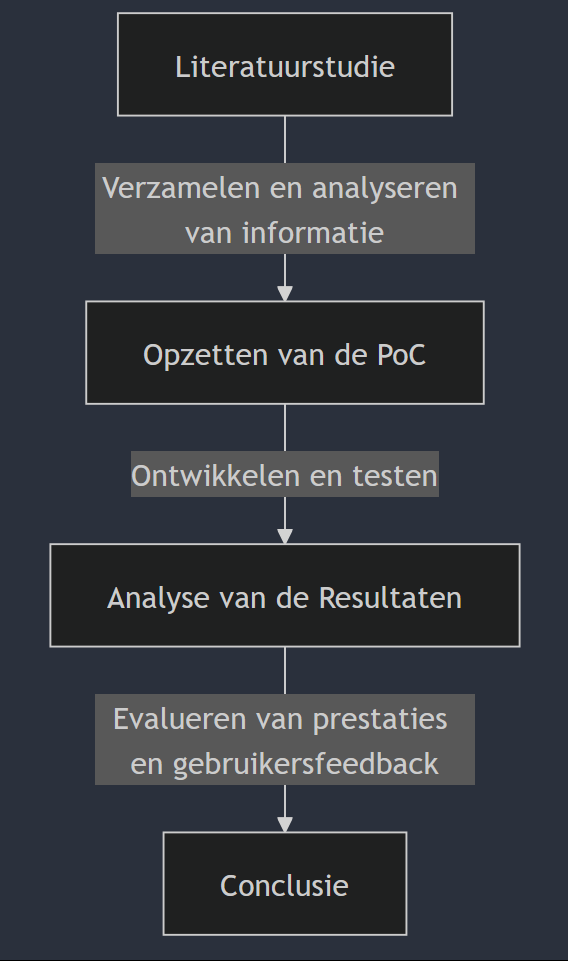
\includegraphics[width=0.7\linewidth]{graphics/flowchart}
    \caption{flowchart}
    \label{fig:flowchart}
\end{figure}

%---------- Verwachte resultaten ----------------------------------------------
\section{Verwacht resultaat, conclusie}%
\label{sec:verwachte_resultaten}
Dit onderzoek moet leiden tot een efficiënter en eenvoudiger gebruik van de software van TurnUp. De klanten zullen Google Agenda kunnen gebruiken om een gecentraliseerde agenda te hebben. 
Ze zullen geen nood meer hebben aan verschillende agenda's.
Dit zal de software van TurnUp ook een boost geven aangezien de efficiëntie van hun product stijgt dankzij dit onderzoek. 



%%---------- Andere bijlagen --------------------------------------------------
% TODO: Voeg hier eventuele andere bijlagen toe. Bv. als je deze BP voor de
% tweede keer indient, een overzicht van de verbeteringen t.o.v. het origineel.
%\input{...}

%%---------- Backmatter, referentielijst ---------------------------------------

\backmatter{}

\setlength\bibitemsep{2pt} %% Add Some space between the bibliograpy entries
\printbibliography[heading=bibintoc]

\end{document}
